\section{功}\label{sec:06.02}

质点的一定的运动状态具有一定的动能。质点的运动状态变
化,它的动能常常也要随之变化。现在我们定义动能的变化过程
为作功,动能的变化量作为功的数量。若在$ t_1 $时刻,质点的动能
为$ T _ { 1 } $;在$ t_2 $时刻,变化到$ T_2 $,则在$ t _ { 1 } $与$ t _ { 2 } $之间的时间里,作功
% 171.jpg
的数量为
\begin{equation}\label{eqn:06.02.01}
 A = T _ { 2 } - T _ { 1 }
\end{equation}
它的物理意义是,要使质点的动能从$ T_1 $变到$ T_2 $,就要对质点作
功。若$ T _ { 2 } > T _ { 1 } $,即质点动能增加,作功为正;若$ T _ { 2 } < T _ { 1 } $,即质点
动能减小,作功为负。

沿用运动学中的方法,我们可以定义动能的平均变化率:
\begin{equation}\label{eqn:06.02.02}
 \langle P \rangle = \frac { T _ { 2 } - T _ { 1 } } { t _ { 2 } - t _ { 1 } } = \frac { \Delta T } { \Delta t }
\end{equation}
$ \langle P \rangle $称为$ t _ { 1 } $到$ t _ { 2 } $时间间隔内的平均功率。同样,瞬时功率定义为
\begin{equation}\label{eqn:06.02.03}
 P = \lim _ { \Delta t \to 0 } \frac { \Delta T } { \Delta t } = \frac { \dif T } { \dif t }
\end{equation}

为了弄清功、功率与他力学量之间的关系,我们首先来讨
\begin{figurex}
    \centering
    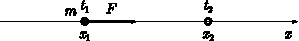
\includegraphics{figure/fig06.04}
    \caption{质点在力作用下的一维运动}
    \label{fig:06.04}
\end{figurex}
论一维直线运动。如图\ref{fig:06.04}\;所示,质量为$ m $的质点在沿$ x $方向的力
$ \vec{F} $作用下,$ t _ { 1 } $时刻在$ x _ { 1 } $ 处,$ t _ { 2 } $时刻运动到$ x _ 2 $。根据牛顿第二定律,有
\begin{equation*}
 m \frac { \dif v } { \dif t } = F
\end{equation*}
两边同乘$ v $,得
\begin{equation*}
 m v \frac { \dif v } { \dif t } = F v
\end{equation*}
亦即
\begin{equation*}
 \frac { \dif } { \dif t } \left( \frac { 1 } { 2 } m v ^ { 2 } \right) = F v
\end{equation*}
或
\begin{equation*}
 \frac { \dif T } { \dif t } = F v
\end{equation*}
所以
\begin{equation}\label{eqn:06.02.04}
 P = F v
\end{equation}
式\eqref{eqn:06.02.04}就是一维情形下的功率、力、速度三者间的普遍关系。
% 172.jpg

由功的定义,显然有
\begin{equation}\label{eqn:06.02.05}
 A = \int _ { t _ { 1 } } ^ { t _ { 2 } } P \dif t
\end{equation}
利用式\eqref{eqn:06.02.04},得
\begin{equation*}
 A = \int _ { t _ { 1 } } ^ { t _ { 2 } } F v \dif t = \int _ { t _ { 1 } } ^ { t_ { 2 } } F \frac { \dif x } { \dif t } \dif t
\end{equation*}
所以\vspace{-1em}
\begin{equation}\label{eqn:06.02.06}
 A = \mathop{\int _ { x _ { 1 } } ^ { x _ { 2 } }}\limits _ { ( l ) } F \dif x
\end{equation}
式\eqref{eqn:06.02.05}及式\eqref{eqn:06.02.06}表示质点在$ t_1 $到$ t_2 $时间间隔里,或从$ x_1 $运
动到$ x_2 $的过程中所涉及的功。因此,从上式我们进一步看清,作
功必定涉及到一个过程。功是度量过程的物理量,它与速度、加
速度、能量等度量物体瞬时性的物理量有很大差别。谈某一瞬时
或某一点的功,是没有意义的。式\eqref{eqn:06.02.06}中积分限的写法,就是
为了表达功是过程量,要对运动的过程积分。譬如图\ref{fig:06.05}\;中,若质
\begin{wrapfigure}[3]{l}{17em}
    \centering
    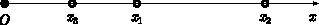
\includegraphics{figure/fig06.05}
    \caption{积分的过程}
    \label{fig:06.05}
\end{wrapfigure}
点运动的过程是从$ x_1 $到$ x_3 $再到$ x_2 $,则积分应由
$ x_1 $到$ x_3 $,再由$ x_3 $到$ x_2 $,
而不是仅由$ x_1 $直接积到$ x_2 $(当然,在特殊条件下,可由$ x_1 $直接积
到$ x_2 $)。

容易将式\eqref{eqn:06.02.04}及式\eqref{eqn:06.02.06}推广到三维情况。这时,牛顿
力学规律是
\begin{equation*}
 m \frac { \dif \vec{ v } } { \dif t } = \vec{F}
\end{equation*}
等式两边点乘$ \vec{ v } $,则有
\begin{equation*}
 m \vec{v} \cdot \frac { \dif \vec{v} } { \dif t } = \vec{F} \cdot \vec{v}
\end{equation*}
或者
\begin{equation*}
 \frac { \dif } { \dif t } \left( \frac { 1 } { 2 } m v ^ { 2 } \right) = \vec{F} \cdot \vec{v}
\end{equation*}
% 173.jpg
因此,代替式\eqref{eqn:06.02.04},是
\begin{equation}\label{eqn:06.02.07}
 P = \vec{F} \cdot \vec{v}
\end{equation}
代替式\eqref{eqn:06.02.06},是
\begin{equation*}
 A = \int _ { t _ { 1 } } ^ { t _ { 2 } } P \dif t = \int _ { t _ { 1 } } ^ { t _ { 2 } } \vec{F} \cdot \vec{v} \dif t
\end{equation*}
因为$ \vec{ v } = \frac { \dif \vec{ r } } { \dif t } $,故
\begin{equation}\label{eqn:06.02.08}
 A = \int _ { t _ { 1 } } ^ { t _ { 2 } } \vec{ F } \cdot \frac { \dif \vec { r } } { \dif t } \dif t = \mathop{\int _ { \vec{r} _ { 1 } } ^ { \vec{r} _ { 2 } }}\limits _ { ( l ) } \vec{F} \cdot \dif \vec{r}
\end{equation}
其中$ (l) $表示沿着质点的运动轨道积分。由式\eqref{eqn:06.02.08}可得,质点
在位移$ \Delta \vec{r} $上,外力$ \vec{F} $作功等于
\begin{equation}\label{eqn:06.02.09}
 \Delta A = \vec{F} \cdot \Delta \vec{r} = |\vec{F}| |\Delta \vec{r}| \cos \theta
\end{equation}
其中$ \theta $是力$ \vec{F} $与位移$ \Delta \vec{r} $之间的夹角。